\documentclass[12pt]{article}
\usepackage{graphicx}
\begin{document}
\parindent=0pt
\setlength{\textwidth=7.0 in}
\setlength{\oddsidemargin=0.00 in}
\setlength{\topmargin=0 in}
\setlength{\textheight=9.5 in}
\centerline{\bf{DUNE Resource Report}}\vskip 1 in \par Configuration: Parameters\_2021-04-28-EB.json\\  Date: 2021-04-28 18:24TZ\\   \\  Fiscal year starts: April 1\\ 
Tape is accounted for at: end of fiscal year\\ 
Disk is accounted for on: October 1\\ 
CPU is accounted for at: end of fiscal year\\ 
Reco passes per Year: 1\\
Sim passes per Year: 1\\
Analysis relative to Sim+Reco: 1\\
\pagebreak
\\
{\bf For data type Raw}\\
   Raw Tape lifetime 100.0 in years\\
   Raw Tape Copies   2.0\\
   Raw FNAL Tape fraction for PD  0.50\\
   Raw FNAL Tape fraction for DUNE  0.50\\
   Raw CERN Tape fraction for PD  0.50\\
   Raw CERN Tape fraction for DUNE  0.00\\
   Raw Collaboration Tape fraction for PD  0.00\\
   Raw Collaboration Tape fraction for DUNE  0.50\\
   Raw Disk lifetime   1.0 in years\\
   Raw Disk Copies   1.0\\
   Raw FNAL Disk fraction for PD  0.50\\
   Raw FNAL Disk fraction for DUNE  1.00\\
   Raw CERN Disk fraction for PD  0.50\\
   Raw CERNDisk fraction for DUNE  0.00\\
   Raw Collaboration Disk fraction for PD  0.00\\
   Raw Collaboration Disk fraction for DUNE  0.00\\
\\
{\bf For data type Test}\\
  Test Tape lifetime   0.5 in years\\
  Test Tape Copies   1.0\\
  Test FNAL Tape fraction for PD  0.50\\
  Test FNAL Tape fraction for DUNE  0.50\\
  Test CERN Tape fraction for PD  0.50\\
  Test CERN Tape fraction for DUNE  0.00\\
  Test Collaboration Tape fraction for PD  0.00\\
  Test Collaboration Tape fraction for DUNE  0.50\\
  Test Disk lifetime   0.5 in years\\
  Test Disk Copies   0.5\\
  Test FNAL Disk fraction for PD  0.50\\
  Test FNAL Disk fraction for DUNE  0.50\\
  Test CERN Disk fraction for PD  0.50\\
  Test CERNDisk fraction for DUNE  0.00\\
  Test Collaboration Disk fraction for PD  0.00\\
  Test Collaboration Disk fraction for DUNE  0.50\\
\\
{\bf For data type Reco}\\
  Reco Tape lifetime  15.0 in years\\
  Reco Tape Copies   1.0\\
  Reco FNAL Tape fraction for PD  0.75\\
  Reco FNAL Tape fraction for DUNE  0.50\\
  Reco CERN Tape fraction for PD  0.00\\
  Reco CERN Tape fraction for DUNE  0.00\\
  Reco Collaboration Tape fraction for PD  0.25\\
  Reco Collaboration Tape fraction for DUNE  0.50\\
  Reco Disk lifetime   2.0 in years\\
  Reco Disk Copies   2.0\\
  Reco FNAL Disk fraction for PD  0.25\\
  Reco FNAL Disk fraction for DUNE  0.25\\
  Reco CERN Disk fraction for PD  0.00\\
  Reco CERNDisk fraction for DUNE  0.00\\
  Reco Collaboration Disk fraction for PD  0.75\\
  Reco Collaboration Disk fraction for DUNE  0.75\\
\\
{\bf For data type Sim}\\
   Sim Tape lifetime  15.0 in years\\
   Sim Tape Copies   1.0\\
   Sim FNAL Tape fraction for PD  0.75\\
   Sim FNAL Tape fraction for DUNE  0.50\\
   Sim CERN Tape fraction for PD  0.00\\
   Sim CERN Tape fraction for DUNE  0.00\\
   Sim Collaboration Tape fraction for PD  0.25\\
   Sim Collaboration Tape fraction for DUNE  0.50\\
   Sim Disk lifetime   2.0 in years\\
   Sim Disk Copies   2.0\\
   Sim FNAL Disk fraction for PD  0.25\\
   Sim FNAL Disk fraction for DUNE  0.25\\
   Sim CERN Disk fraction for PD  0.00\\
   Sim CERNDisk fraction for DUNE  0.00\\
   Sim Collaboration Disk fraction for PD  0.75\\
   Sim Collaboration Disk fraction for DUNE  0.75\\
\begin{table}
\footnotesize
 \centering \begin{tabular}[h]{crrrrrcccc}
 & CPU &Wall&Wall F/C&\qquad  & Tape\qquad& Tape\qquad  & Disk\qquad  & Disk\qquad \\
Years&(Mhrs)&kSPEC06&kSPEC06&cores& Total(PB)&F/C/Collab & Total(PB) &F/C/Collab\\
\hline
2020&	  30&	  54&	  14/  41&	  4915&	     14.2&	   9.1/  3.0/  2.1&	     15.4&	   4.0/  0.4/ 10.9\\
2021&	  40&	  73&	  18/  54&	  6594&	     21.3&	  14.1/  3.7/  3.5&	     20.5&	   5.3/  0.5/ 14.7\\
2022&	  64&	 115&	  29/  86&	 10443&	     39.6&	  25.4/  8.6/  5.6&	     33.6&	   9.7/  2.6/ 21.3\\
2023&	  73&	 130&	  33/  98&	 11835&	     52.7&	  34.3/ 10.5/  7.9&	     38.3&	  10.3/  1.4/ 26.6\\
2024&	  70&	 125&	  31/  94&	 11373&	     61.7&	  41.0/ 10.5/ 10.2&	     36.9&	   9.3/  0.1/ 27.5\\
2025&	  29&	  53&	  13/  40&	  4795&	     65.7&	  44.0/ 10.5/ 11.2&	     26.3&	   6.6/  0.1/ 19.5\\
2026&	  29&	  52&	  13/  39&	  4729&	     70.9&	  47.8/ 10.6/ 12.4&	     18.2&	   4.6/  0.2/ 13.4\\
2027&	  29&	  52&	  13/  39&	  4729&	     80.3&	  40.1/  0.0/ 40.1&	     22.2&	   6.2/  0.0/ 16.0\\
2028&	  46&	  83&	  21/  63&	  7583&	     95.8&	  47.9/  0.0/ 47.9&	     31.8&	  11.5/  0.0/ 20.3\\
2029&	  54&	  98&	  24/  73&	  8888&	    113.6&	  56.8/  0.0/ 56.8&	     40.1&	  13.9/  0.0/ 26.2\\
2030&	  68&	 122&	  30/  91&	 11089&	    139.5&	  69.7/  0.0/ 69.7&	     48.3&	  18.8/  0.0/ 29.5\\
2031&	  82&	 146&	  37/ 110&	 13291&	    161.3&	  80.7/  0.0/ 80.7&	     50.8&	  18.8/  0.0/ 32.0\\
2032&	  95&	 170&	  43/ 128&	 15492&	    195.0&	  97.5/  0.0/ 97.5&	     58.5&	  21.4/  0.0/ 37.1\\
2033&	 114&	 205&	  51/ 153&	 18591&	    231.8&	 115.9/  0.0/115.9&	     68.2&	  26.7/  0.0/ 41.5\\
2034&	 133&	 239&	  60/ 179&	 21689&	    262.6&	 131.3/  0.0/131.3&	     72.2&	  27.0/  0.0/ 45.1\\
2035&	 152&	 273&	  68/ 205&	 24788&	    304.9&	 152.5/  0.0/152.5&	     81.4&	  30.0/  0.0/ 51.4\\
2036&	 176&	 317&	  79/ 237&	 28783&	    349.9&	 175.0/  0.0/175.0&	     92.6&	  35.7/  0.0/ 57.0\\
2037&	 201&	 361&	  90/ 270&	 32779&	    389.1&	 194.5/  0.0/194.5&	     98.2&	  36.4/  0.0/ 61.8\\
2038&	 226&	 405&	 101/ 303&	 36774&	    434.7&	 217.3/  0.0/217.3&	    106.3&	  38.4/  0.0/ 67.9\\
2039&	 250&	 448&	 112/ 336&	 40770&	    482.5&	 241.3/  0.0/241.3&	    114.5&	  40.5/  0.0/ 74.0\\
2040&	 274&	 492&	 123/ 369&	 44765&	    537.5&	 268.7/  0.0/268.7&	    122.7&	  42.5/  0.0/ 80.1\\
\end{tabular}
\caption{Assume present core is   11 SPEC06. CPU number is real CPU. Cores and SPEC06 are Walltime with CPU/Walltime =  0.70.  F means FNAL, C means CERN. Assume CERN storage is only  for ProtoDUNE. CPU should be divided 25\% FNAL, 75\% Collab}\normalsize
 \end{table}
\pagebreak\begin{figure}
\centering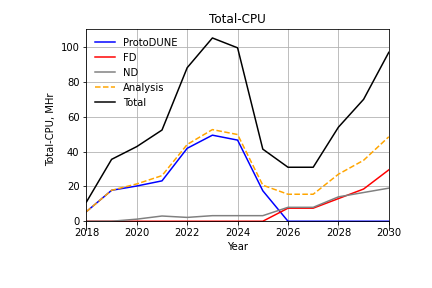
\includegraphics[height=0.4\textwidth]{Total-CPU.png}\label{TotalCPU}
\caption{CPU time in Wall Hours/year}
\end{figure}
\begin{figure}
\centering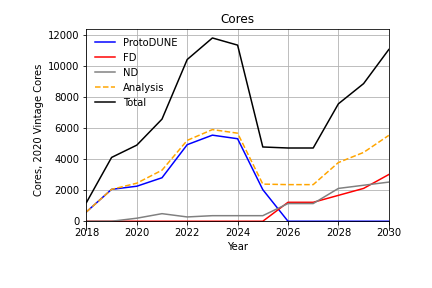
\includegraphics[height=0.4\textwidth]{Cores.png}\label{Cores}
\caption{Cores needed, including efficiency loss}
\end{figure}
\begin{figure}
\centering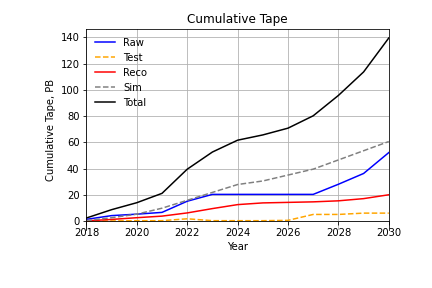
\includegraphics[height=0.4\textwidth]{Cumulative-Tape.png}\label{CumulativeTape}
\caption{Tape tape needs, PB, all types are cumulative over tape lifetime}
\end{figure}
\begin{figure}
\centering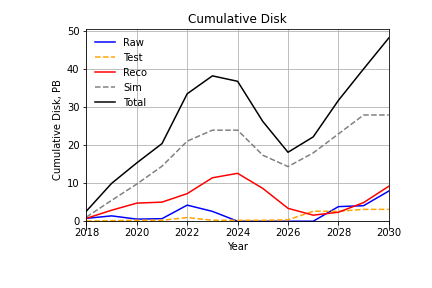
\includegraphics[height=0.4\textwidth]{Cumulative-Disk}\label{CumulativeDisk}
\caption{Disk needs, PB.  Reco and Sim are cumulative over disk lifetime.  Raw and Test have sub-year lifetimes.}
\end{figure}
\vskip 3 in\pagebreak 
 {\bf Change log:}\\
2021-04-27 change HSPEC06 to 11 from 15 per CMS numbers from Kirby\\2021-04-21 clarify CERN vs Collab for first 10 years\\2021-03-26 clearer plots, go to v3 of the code to preserve the RRB code in v2\\2021-03-24 try with CERN/FNAL combined for raw and test.\\2021-03-22 add Collab vs FNAL shares, restore sim disk lifetime to 2.\\\end{document}